% !TeX spellcheck = en_GB
\subsubsection{Event Selection}\label{section:star_event_selection}
Events were selected from those passing the SDT trigger condition. In order to remove events of poor quality and to suppress background the following conditions were required:
\begin{enumerate}
	\item trigger signals in exactly two stations of one arm of \ac{RP} system (this requirement divides the~sample into four  sub-samples, which were later analysed independently, e.g. for background studies),
	\item any trigger signal in small BBC tiles on the opposite side of the STAR central detector to the~triggered RP station,
	\item exactly one proton track in the above RP stations with $0.02 < \xi < 0.2$ and $0.04 < -t < 0.16$~GeV$^{2}$/c$^{2}$. 
	\item exactly one  vertex  reconstructed from  TPC tracks matched with hits in TOF (later in the~text such vertex  is referred as a TOF vertex),
	\item TOF vertex  within $|V_z|<80$~cm - events with vertices away from the~nominal IP have low acceptance for the central and forward tracks,%~\cite{supplementaryNote},
	\item at least two but no more than eight primary TPC tracks, $2\leq n_{\textrm{sel}}\leq 8$, matched with hits in TOF and satisfying the selection criteria described in Sec.~\ref{section:star_track_selection},
	\item if there are exactly two primary tracks satisfying the~above criteria and exactly two global tracks used in vertex reconstruction (Sec.~\ref{section:star_vertex}), the longitudinal distance between these global tracks should be smaller than $2$~cm, $|\Delta z_0|<2$~cm. %, due to small ($<20\%$) vertex reconstruction efficiency for tracks with $|\Delta z_0|>2$~cm (as described in Sec.~\ref{section:star_vertex}).
\end{enumerate}
Figure~\ref{fig:vertexSTAR} shows the multiplicity of TOF vertices $n_\textrm{vrt}$ (left)  and the $z$-position of  reconstructed vertices in single TOF vertex events (right). Data are compared to embedded PYTHIA~8 SD sample. These distributions are not significantly process-dependent, therefore, contributions from other processes are not included in these plots. Most events with $n_\textrm{vrt} > 1$ originate from in-time pile-up and are excluded from the~analysis.
\begin{figure}[b!]
	\centering
	\includegraphics[width=.49\textwidth, page=13]{chapters/chrgSTAR/img/selection/SDT.pdf}
	\includegraphics[width=.49\textwidth, page=7]{chapters/chrgSTAR/img/selection/SDT.pdf}
	\caption{(left) Vertex multiplicity  and  (right) the~$z$-position of  reconstructed vertices in single TOF vertex events before applying  the~cut on the~quantity shown. Blue lines indicate regions accepted in the analysis.}
	\label{fig:vertexSTAR}
\end{figure}
\subsubsection{ZDC Veto}\label{section:star_zdc_selection}
The~SDT trigger conditions imposed a veto on any signal in the~same-side ZDC. However, all MC samples do not contain ZDC simulation. To check the impact of this veto on the measurement, the total energy of neutral particles, such as $n$, $\gamma$, $\pi^{0}$, produced within ZDC acceptance ($|\eta|>6$) was measured using true-level PYTHIA~8~(SaS). In most of the events, the~energy measured on the proton side of the~IP is smaller than trigger thresholds (as shown in Fig.~\ref{fig:zdcSTAR}). Therefore, the~ZDC veto has a~negligible effect on the~analysis and ZDC simulation is not needed.


\begin{figure}[t!]
	%\vspace{-1cm}
	\centering
	\begin{subfigure}{.45\textwidth}
		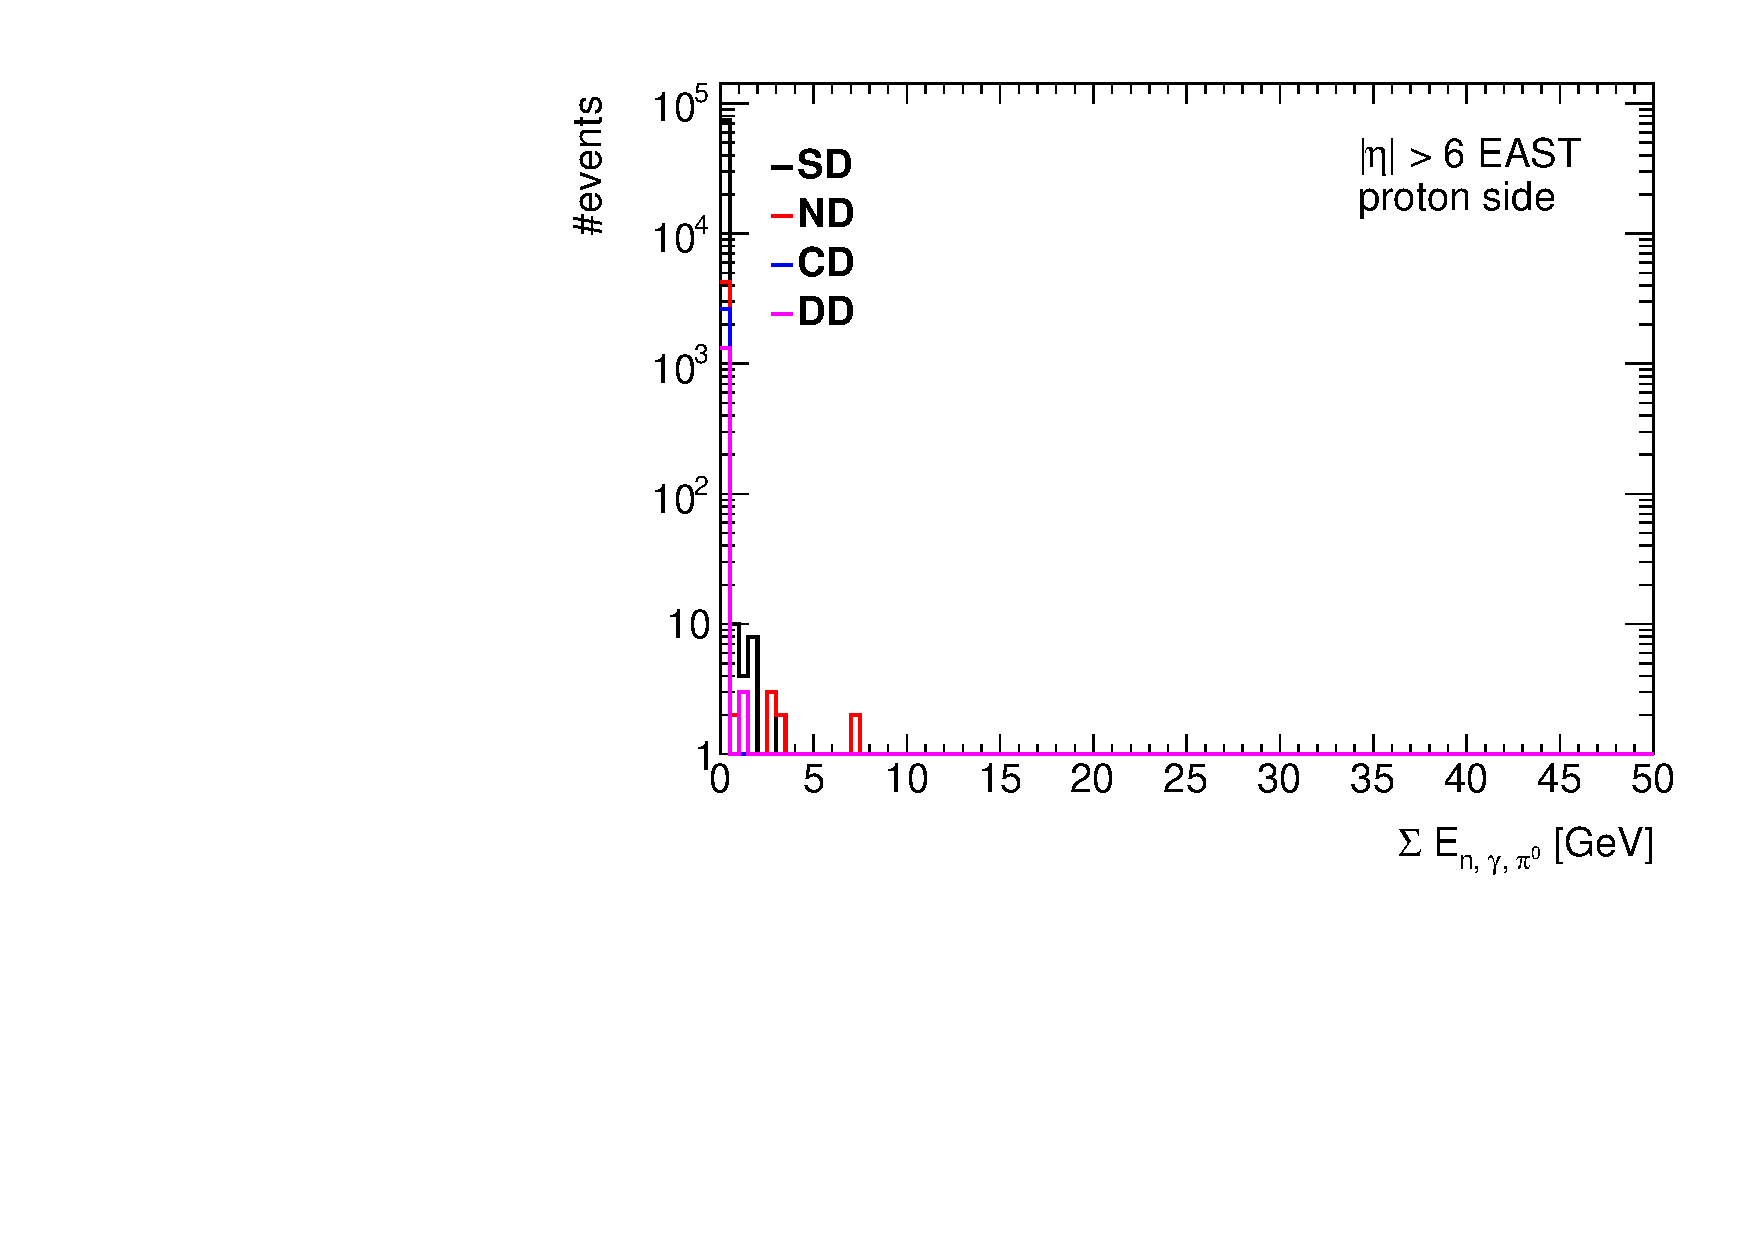
\includegraphics[width=\textwidth, page=1]{chapters/chrgSTAR/img/zdc/out.pdf}
		%\caption{}
	\end{subfigure}
	\begin{subfigure}{.45\textwidth}
		\includegraphics[width=\textwidth, page=2]{chapters/chrgSTAR/img/zdc/out.pdf}
		%\caption{}
	\end{subfigure}
	\begin{subfigure}{.45\textwidth}
		\includegraphics[width=\textwidth, page=3]{chapters/chrgSTAR/img/zdc/out.pdf}
		%\caption{}
	\end{subfigure}
	\begin{subfigure}{.45\textwidth}
		\includegraphics[width=\textwidth, page=4]{chapters/chrgSTAR/img/zdc/out.pdf}
		%\caption{}
	\end{subfigure}
	%\begin{minipage}{.45\textwidth}
		
		
		\caption{Total energy of neutral particles ($n$, $\gamma$, $\pi^{0}$) produced within ZDC acceptance ($|\eta|>6$) for events in which forward-scattered proton is on (top) west and (bottom) east side of the~IP. Distributions are presented separately for neutral particles produced on  (left) the proton and (right) opposite side of the IP. PYTHIA~8 predictions for different processes are shown as colour histograms. }
		\label{fig:zdcSTAR}
	%\end{minipage}
\end{figure}
%\FloatBarrier